\externaldocument{../appendix/chapter_app}
\externaldocument{../4/chapter_algorithm}
\externaldocument{../3/chapter_modeling}
\startchapter{Proof of Concept}
\label{chapter:Exp}
In this section, I present two experiments I ran as a proof of concept of the communication analysis of two traces.

These experiments aimed to test the communication model and the communication analysis approach. They also verify the design of the some algorithms, for their correctness. I used the implemented features on Atlantis to conduct the experiments.

Among these two experiments, the first one was provided directly by our research partner DRDC with their initial requirement, while the second one was designed by me. In both experiments, DRDC conducted the programs execution and captured the traces on their environment while I performed the analysis locally with Atlantis on my desktop with the captured traces and corresponding .dll.

All test programs in these two experiments were written in C++ and the source code can be found in Appendix \ref{expcode}. Results are provided for each experiment. 

Both of the conducted experiments used the named pipe communication method. The reason that I only perform the experiments related to named pipe is that the in-house tracer of DRDC can only support capturing the function information for named pipe function calls at the time when I was performing the experiments. 


I will describe the design of the experiments first. And then, I present the result of them following by the discussion.

\section{Experiment 1}
\subsection{Experiment Design}
In the first experiment, two programs communicated with each other through a synchronous named pipe channel. One of the programs acted as the named pipe server while the other as the client. Figure \ref{exp1} is the sequence diagram of the interaction between the server and client. This sequence diagram only exemplify a possible sequence of the events. The actual events sequence can vary depending on the run-time environment. 


\begin{figure}[H]
\centerline{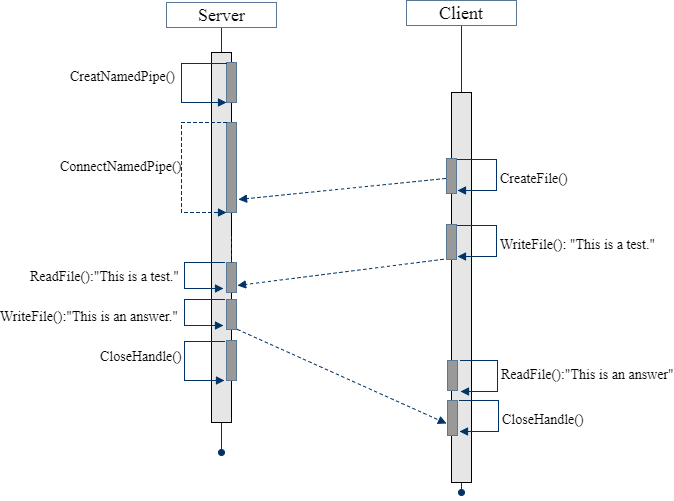
\includegraphics[scale=0.7]{Figures/exp1}}
 \caption{Sequence Diagram of Experiment 1}
\label{exp1}
\end{figure}

Two traces were captured while these two programs were running and interacting. The two captured traces, ``Sever.trace" and ``Client.trace" were analyzed as dual\_trace in this experiment. I used the implemented features in Atlantis to analyze this dual\_trace. I ran the ``Stream identification" and ``Communication identification" operations for this dual\_trace. 

\subsection{Dual\_trace Analysis Result}
The extracted streams and identified communications of the dual\_trace in this experiment are showed in Figure\ref{result1}.

\begin{figure}[H]
\centerline{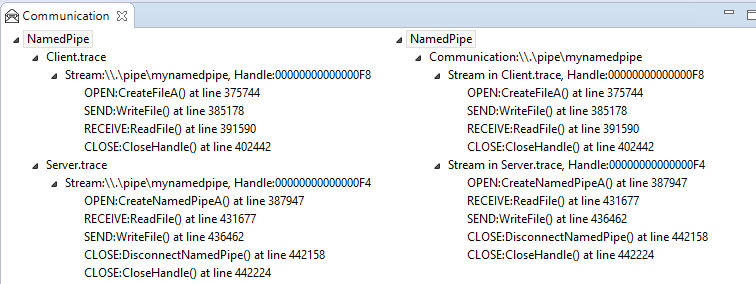
\includegraphics[scale=0.65]{Figures/result1}}
 \caption{Analysis Result of Dual\_trace in Experiment 1}
\label{result1}
\end{figure}

\subsection{Discussion}
In the result of $exp1$, there are one stream extracted in client trace and one in server trace, and these two streams are matched into a communication of this dual\_trace. This identification result represents the actual communication happen between the named pipe server and client.
In the result of $exp2.1$ and $exp2.2$, there are one stream in each of the client traces and four in the server trace respectively. The streams are further matched and verified and eventually one communication is identified for each dual\_trace. The result aligns to the sequence diagram in Figure\ref{exp2}.

\section{Experiment 2}
\subsection{Experiment Design}
In the second experiment, a program was running as the named pipe server. In this server program, four named pipes were created and can be connected by up to four client at a time. Two other programs as the named pipe clients connected to this server. Those two clients (client 1 and client 2) used the identical program but run in sequence. Figure \ref{exp2} is the sequence diagram of the interaction among the server and clients. This sequence diagram only exemplify a possible sequence of the events. The actual events sequence can vary depending on the run-time environment. 

\begin{figure}[H]
\centerline{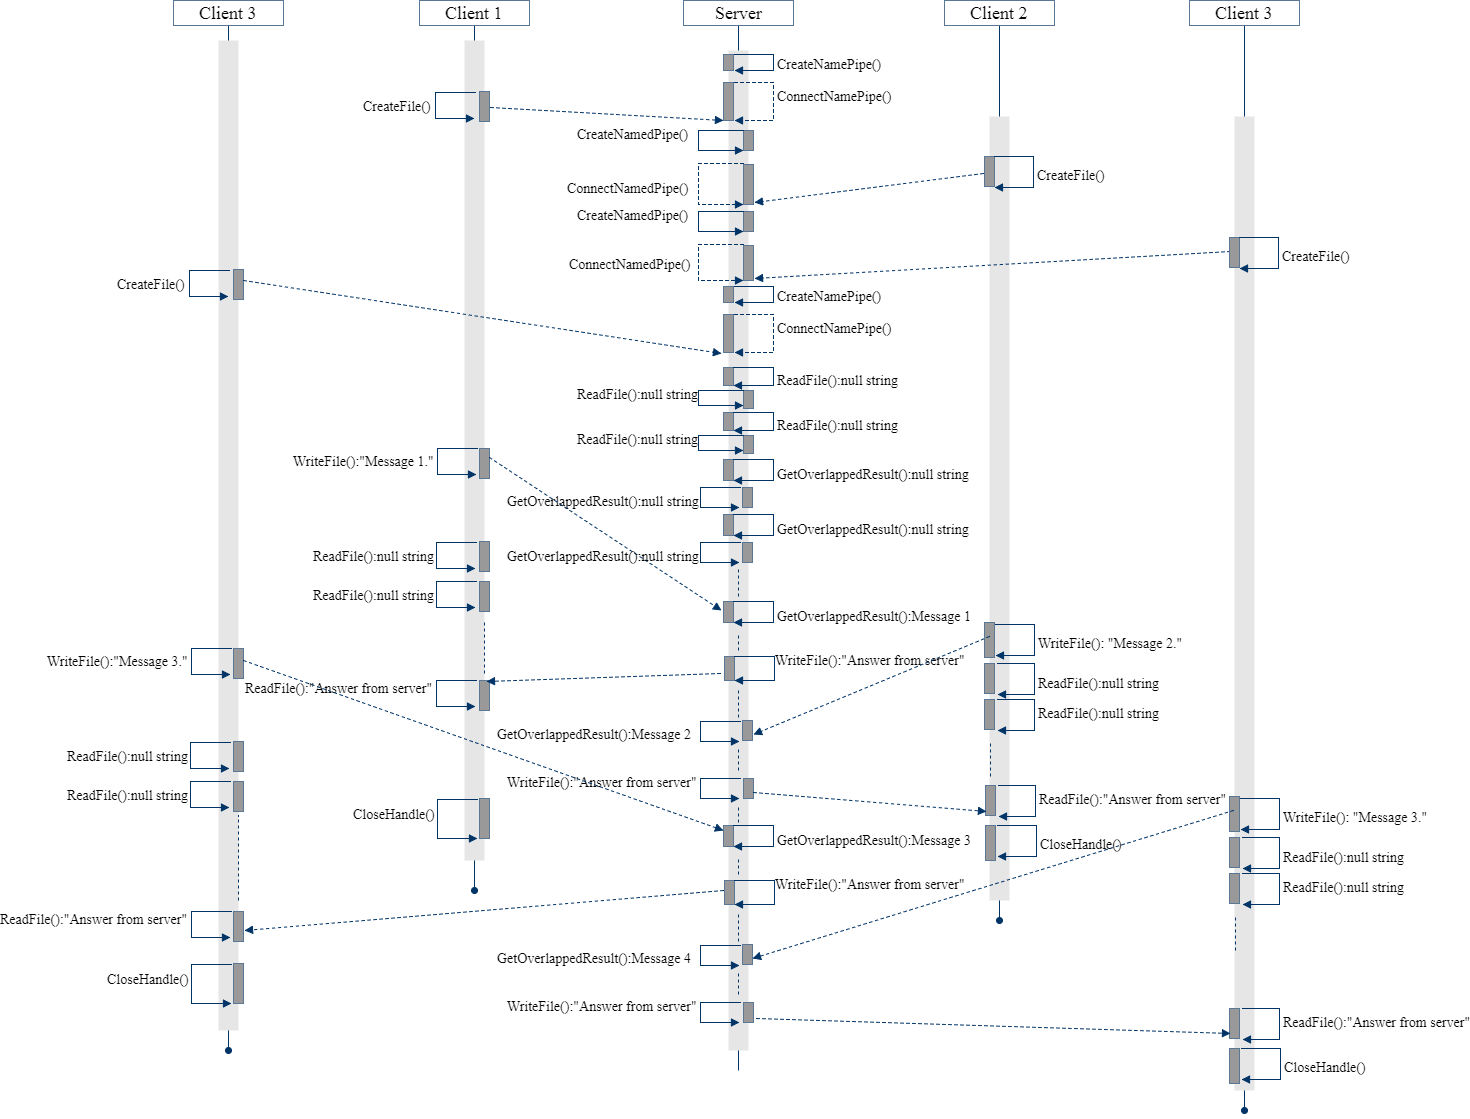
\includegraphics[scale=0.6]{Figures/exp2}}
 \caption{Sequence Diagram of Experiment 2}
\label{exp2}
\end{figure}

Three traces were captured at the time when these three programs were running and interacting. They are ``Server.trace" for the server program, ``Client1.trace" for the Client1 program and ``Client2.trace" for the Client2 program. These three traces are analyzed as two dual\_traces, one consist of ``Server.trace" and ``Client1.trace" while the other consist of ``Server.trace" and ``Client2.trace". I performed the ``Stream Extraction" and ``Communication Identification" operations for these two dual\_traces. 

\subsection{Dual\_trace Analysis Result}
The extracted streams and identified communications from the two dual\_traces are shown in Figure \ref{result21} and Figure \ref{result22}.

\begin{figure}[H]
\centerline{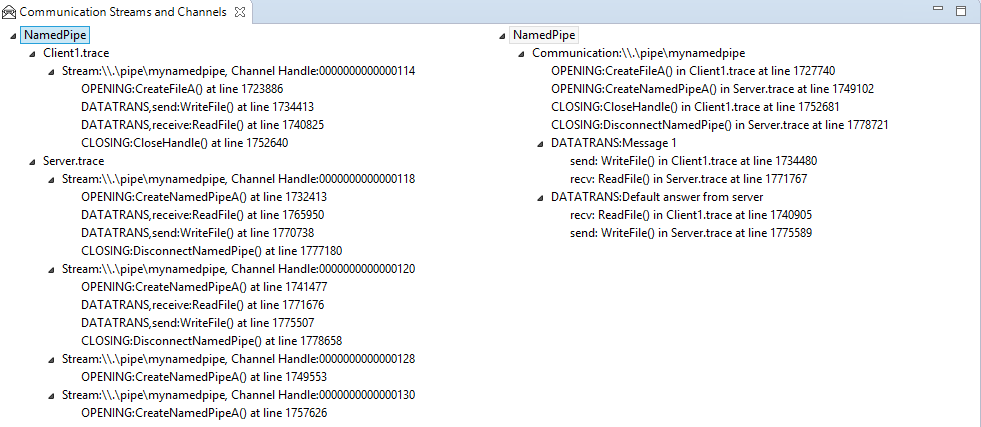
\includegraphics[scale=0.55]{Figures/result21}}
 \caption{Analysis Result of the Dual\_trace:``Server.trace" and ``Client1.trace" in Experiment 2}
\label{result21}
\end{figure}

\begin{figure}[H]
\centerline{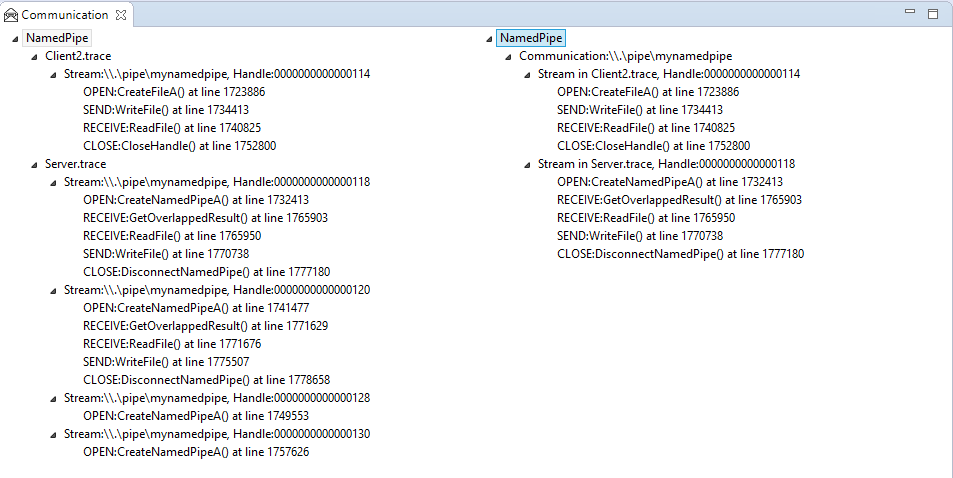
\includegraphics[scale=0.55]{Figures/result22}}
 \caption{Analysis Result of the Dual\_trace:``Server.trace" and ``Client2.trace" in Experiment 2}
\label{result22}
\end{figure}


\subsection{Discussion}
In the result of $exp1$, there are one stream extracted in client trace and one in server trace, and these two streams are matched into a communication of this dual\_trace. This identification result represents the actual communication happen between the named pipe server and client.
In the result of $exp2.1$ and $exp2.2$, there are one stream in each of the client traces and four in the server trace respectively. The streams are further matched and verified and eventually one communication is identified for each dual\_trace. The result aligns to the sequence diagram in Figure\ref{exp2}.


   




